\documentclass[10pt,twocolumn,letterpaper]{article}

\usepackage{cvpr}
\usepackage{times}
\usepackage{epsfig}
\usepackage{graphicx}
\usepackage{amsmath}
\usepackage{amssymb}

% Include other packages here, before hyperref.

% If you comment hyperref and then uncomment it, you should delete
% egpaper.aux before re-running latex.  (Or just hit 'q' on the first latex
% run, let it finish, and you should be clear).
\usepackage[pagebackref=true,breaklinks=true,letterpaper=true,colorlinks,bookmarks=false]{hyperref}


% \cvprfinalcopy % *** Uncomment this line for the final submission

\def\cvprPaperID{****} % *** Enter the 3DIMPVT Paper ID here
\def\httilde{\mbox{\tt\raisebox{-.5ex}{\symbol{126}}}}

% Pages are numbered in submission mode, and unnumbered in camera-ready
\ifcvprfinal\pagestyle{empty}\fi
\begin{document}

%%%%%%%%% TITLE
\title{\LaTeX\ Author Guidelines for 3DIMPVT Proceedings}

\author{First Author\\
  Institution1\\
  Institution1 address\\
  {\tt\small firstauthor@i1.org}
  % For a paper whose authors are all at the same institution, omit
  % the following lines up until the closing ``}''.  Additional
  % authors and addresses can be added with ``\and'', just like the
  % second author.  To save space, use either the email address or
  % home page, not both
  \and
  Second Author\\
  Institution2\\
  First line of institution2 address\\
  {\small\url{http://www.author.org/~second}} }

\maketitle
% \thispagestyle{empty}

%%%%%%%%% ABSTRACT
\begin{abstract}
  Automated 3D modeling of building interiors is useful in applications
  such as virtual reality and environment mapping. Accurate texture
  mapping of these models is vital towards visualizing the data
  gathered by modeling systems and increases overall usability. The
  localization of cameras in 3D scenes often suffers from inaccuracies, resulting in visible discontinuties
  when images are directly projected onto a plane for
  texturing. Previous approaches at minimizing these discontinuities
  do not robustly handle a wide range of camera locations and angles, and often suffer from error accumulation when stitching together multiple
  images. We propose two variants on a new approach for reducing discontinuities
  during texture mapping, one tailored for optimal images, and one tailored for sub-optimal images.
\end{abstract}

%%%%%%%%% BODY TEXT
\section{Introduction}
Three-dimensional modeling of indoor environments has a variety of
applications such as training and simulation for disaster management,
virtual heritage conservation, and mapping of hazardous sites. Manual
construction of these digital models can be time consuming, and as
such, automated 3D site modeling has garnered much interest in recent
years.

The first step in automated 3d modeling is the physical scanning of
the environment's geometry. An indoor modeling system must be able to
calculate camera locations within an environment while simulatenously
reconstructing the 3D structure of the environment itself. This
problem is studied by the robotics and computer vision communities as
the simultaneous localization and mapping (SLAM) problem, and is
generally solved using a combination of laser range scanners, cameras,
and inertial measurement units (IMUs).

The aim of this paper is to present a solution for texture mapping the
3D models generated by indoor modeling systems, with specific
attention given to a human-operated system with higher localization
errors and greater variance in camera locations. The paper is
organized as follows. Section \ref{sec:backpackSystem} provides an
overview of the backpack modeling system from which data and examples
used throughout this paper originate. Section
\ref{sec:textureMappingOverview} describes the general problem of 3D
texture mapping and reviews existing approaches. Section
\ref{sec:textureMappingMethods} describes our new approach towards texture mapping, as well as unique challenges posed by the
backpack modeling system and our two approaches tailored for
walls and floors/ceilings respectively. Section \ref{sec:results}
compares results and presents conclusions.

\section{Backpack Modeling System}
\label{sec:backpackSystem}
Human-operated data acquisition systems provide unique advantages over
vehicular-mounted systems in terms of agility and
portability. Unfortunately, human-operated systems also suffer from a
lack of automation and stability, often resulting in much higher data
variance and localization error. As a result, common methods for
texture mapping often produce poor results, as examined in section
XX. Before discussing how to overcome these challenges, we will first
provide an overview of the backpack modeling system from which our
test data was obtained.

\subsection{Data Acquisition Hardware}
\label{sec:backpackHardware}
The backpack modeling system which we worked with contains five 2D
laser range scanners, two cameras, an orientation sensor, and an
IMU. The laser scanners have a 30-meter range and a 270$^{\circ}$
field of view. The two cameras are equipped with fisheye lenses,
resulting in a 180$^{\circ}$ field of view, and are mounted with one
facing left and one facing right. The IMU provides highly accurate
measurements of all 6 DOF at 200Hz, and is used as a ground truth
reference. The orientation sensor provides orientation parameters at a
rate of 180Hz.

With this backpack actively scanning, a human operator then takes
great care to walk a path such that every wall in the desired indoor
environment is passed and scanned lengthwise at least once.

\subsection{Environment Reconstruction}
\label{sec:environmentReconstruction}
Using data gathered by the onboard sensors and multiple localization
and loop-closure algorithms, the backpack is localized over its data
collection period, and a 3D point cloud of the surrounding environment
is constructed based on the laser scanner readings. Approximate normal
vectors for each point in the point cloud are then calculated by
gathering neighboring points within a small radius and processing them
using principal component analysis. These normal vectors allow for the
classification and grouping of adjacent points into structures such as
walls, ceilings, floors, and staircases. A RANSAC algorithm is then
employed to fit polygonal planes to these structured groupings of
points, resulting in a fully planar model. This planar model,
consisting of multiple 2D polygonal planes in 3D space, must then be
textured by all or some subset of the images captured by the
backpack's camera.


\subsection{Image Association}
\label{sec:imageAssociation}
Before discussing texture mapping, we (something goes here based on whether we take credit for stewarts work or not)


In order to speed up our texture mapping process, it is prudent to
reduce the amount of potential images being considered for texture
mapping each plane. The backpack modeling system takes 5
pictures/second from both cameras, resulting in each plane being
present in (and capable of being textured mapped by) thousands of
images, at a wide range of distances and angles. Thus, for the sake of
efficiency, it makes sense to associate each plane with a much smaller
list of images, preferably some set which contains the most desirable images
according to some metric. Thus we keep three criteria in mind while
selecting such a subset. First, we want our final collection of images
to be capable of covering the entirety of a plane, so as to ensure
there are no holes in our final texture. Second, we want all our
images to be taken from a relatively close distance to the plane, and
at as much of a direct, head-on angle as possible. This ensures that
the image projects squarely onto our desired plane, with minimal
inclusion of other planes, and we end with a texture with high
resolution. Third, we desire an amount of overlap between the images
chosen. This overlap provides us with a buffer in case we shift images
as discussed in Section X, and is also required for the blending
process presented in Section Y.

To meet these three criteria, we divide each plane into small triangles just a few centimers across. Triangulation is used due to the fairly complex
geometry of many of our planes, and is accomplished by using a
standard ear-clipping algorithm followed by further triangular
tesselation. For each triangle, we gather all images that can be
projected upon the entirety of the triangle, accounting for occlusion
with other planes as well, using standard ray-polygon intersection
tests. Of these images, we then select the best one
according to the heuristic in equation X, which favors closer distances
and more head-on projection angles. We also enforce that no two images
are chosen such that they were taken within 0.5 meters of eachother,
so as to reduce our overall amount of images. The end result is a
greatly-reduced set of images such that each one is objectively a good choice for texturing some number of areas on the plane. Furthermore, since cameras are only at good
angles to triangles near their center of projection, and poor
candidates for triangles near their edges, images will be chosen such
that there is high overlap between successive images. With the three criteria satisfied, we have reduced the amount of candidate images for
each plane from many thousands to around 50-100.

\subsection{Occlusion Checking}
Before we proceed with texturing our planes, we need to ensure that
each plane's associated images contain only content that should be
mapped onto the target plane in question. From the above process,
images were chosen such that they had an unoccluded view of one or
more trianglular sections upon a plane. This may not necessarily hold
true however for all areas of the plane, as demonstrated in figure
SOMETHING. If images are not modified to mask out occluded areas,
different images could attempt to cover the same location on a plane
with drastically different textures, inevitably leading to
undesireable discontinuities in our final texture.

Fortunately, by virtue of our indoor environments, the vast majority
of surface geometry is either horizontal or vertical, with high
amounts of right angles. This means that the areas we wish to mask out
of our images due to occlusion are nearly always rectangular
areas. Similar to the triangular tesselation performed for image
association above, we split each image into rectangular pieces, and
perform occlusion checks for a sampling of points within each
piece. For rectangles with occluded points, we then subdivide them
into smaller rectangles, and repeat the process, until we reach some
manually-set recursion limit. To actually occlude out rectangles, we
simply remove their texture, as untextured areas will never be chosen
for texture mapping. We are now ready to begin the texture mapping
process.

\section{Texture Mapping Overview}
\label{sec:textureMappingOverview}

\begin{figure}
  \centering
  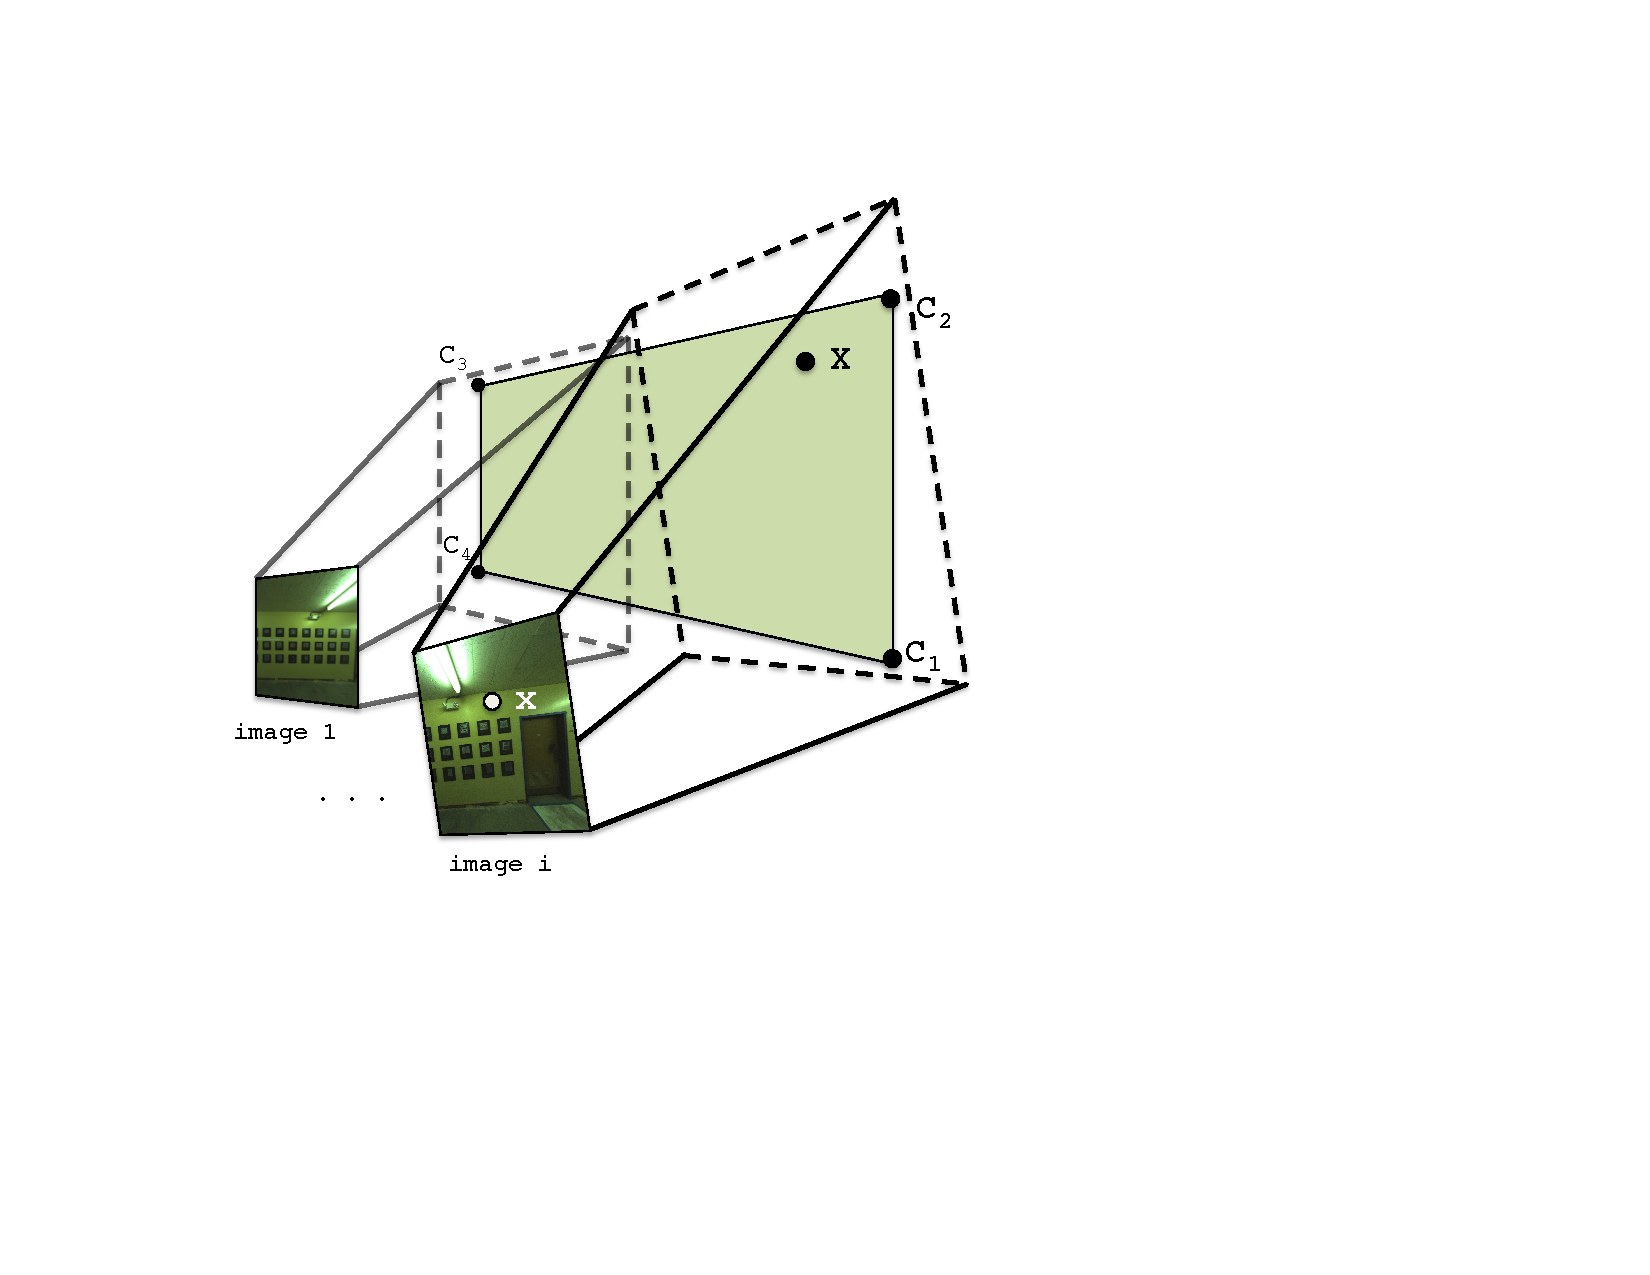
\includegraphics[height=2in]{Projection.pdf}
  \caption{Planes are specified in 3D space by four corners $C_1$ to
    $C_4$. Images are related to each plane through the camera
    matrices $P_{1..M}$. }
  % \caption{The plane is specified in 3D space by the four corners
  % $C_1$ to $C_4$. Images are related to the plane through the camera
  % matrices $P_{1..M}$. For example, the 3D point X in the world
  % coordinate system is related to the image point x shown in the
  % figure as $x = P_i X$.}
  \label{fig:projection}
\end{figure}

In this section, we will discuss the process of texture mapping a
single plane, as the texturing of each of our planes is completely
independent and can be completed in parallel.  

The geometry of the general texture mapping process is shown in Figure 1. 

 As
described in the previous section, we are provided with a set of $M$
images for each plane. Each image has a camera matrix $P_i$ for $i=1..M$, which
translates a 3D point in the world coordinate system to a 2D point in
image $i$'s coordinates. A camera matrix $P_i$ is composed of the
camera's intrinsic parameters, such as focal length and image center,
as well as the extrinsic parameters which specify the rotation and
translation of the camera's position with respect to the world
coordinates at the time that image $i$ was taken. These extrinsic
parameters are determined by the localization hardware and algorithms
mentioned in Section \ref{sec:backpackSystem}. A point $X$ on the
plane in 3D space can be related to its corresponding pixel $x$ in image $i$
through the following equation:

\[
x=project(P_iX)
\]

where
\[X = \begin{pmatrix} x \\ y \\ z \end{pmatrix} \textrm{ and }
project(X) = \begin{pmatrix} x/z \\ y/z \end{pmatrix}
\]

For the sake of simplicity, we treat all planes as rectangles by generating a minimum bounding box for them. Their original vertices can be recovered later as needed, and used to crop any excess texture. A plane to be textured is thus defined by its bounding box with corners $C_i$ in
world coordinates and a normal vector indicating the front facing side
of the plane. Our goal is to texture this plane using its associated
images, while eliminating any visual discontinuities or seams that
would suggest that the plane's texture was not composed of a single
continuous image.



\subsection{Naive Mapping}
\label{sec:naive}
\begin{figure}
  \centering
  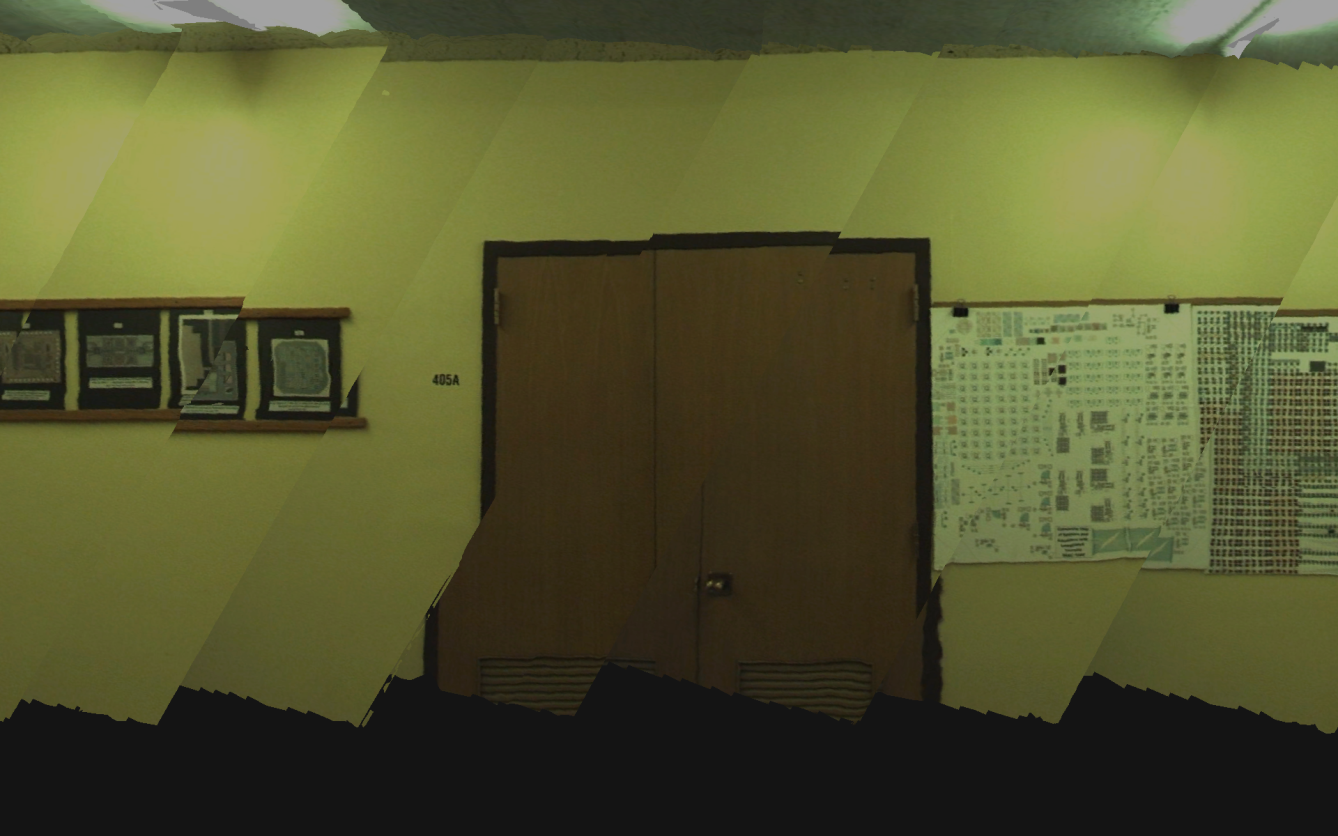
\includegraphics[height=1.5in]{naive.png}
  \caption{The result of naive texture mapping based on the imprecise
    camera matrices estimated by the localization system.}
  \label{fig:naive}
\end{figure}


Ignoring the fact that the camera matrices $P_{1..M}$ are inaccurate,
one can texture map the plane by simply applying textures according to
the image association process and scoring function described in
Section X. This naive mapping approach independently selects the best
texture for each trianglular section on the plane, but it also means
that all of our $M$ images are used for the overall texture, thus
increasing the potential amount of poor image boundaries.

As Figure \ref{fig:naive} demonstrates, this approach leads to many
image boundaries with abrupt discontinuities, due to significant
misalignment between images. One approach also tuned for our datasets
attempted to minimize these discontinuities through more intelligent
image selection, making use of spatial and temporal caching
mechanisms.

\subsection{Mapping with Caching}
In order to reduce the severity of discontinuities between adjacent
triangles, one can texture them with the same image, if possible,
eliminating the discontinuity outright, or by two images taken from
similar positions, such that any texture mismatch is ideally less
pronounced. This is accomplished by adding a 2-level cache to the
native mapping approach, and sorting triangles in an order such that
triangle $t_i$ is adjacent to triangle $t_{i+1}$. When a
triangle is assigned a texture, the image it selected is added to the
level 1 cache, and other images that were taken nearby in time and
location, within a predefined threshold, are added to the level 2
cache. Each subsequent triangle to be textured then searches through
the level 1 cache, selecting the best image according to the same
scoring function, and comparing it to some pre-defined threshold. If
the best image's score is below this threshold, the level 2 cache is
then searched, and then finally if necessary, the set of all images is
searched. In this way, the entire plane is textured, with image reuse prioritized, followed by a preference for nearby images.

This approach is the method previously used by the modeling team
associated with our dataset. Therefore, we will use it as our baseline
when comparing other approaches.  The addition of the caching
structure reduces discontinuities overall, as can be seen in the above
image. Nevertheless, the amount of remaining discontinuities suggests
that image selection alone cannot produce seamless textures.  In order
to produce photorealistic texture mapping, either the camera matrices
need to be refined such that the localization is pixel accurate,
resulting in a perfect mapping, or image stitching techniques need to
be applied to provide this illusion. A commonly-used technique for
each approach is examined next.




\subsection{Image Mosaicing}

\begin{figure}
  \centering
  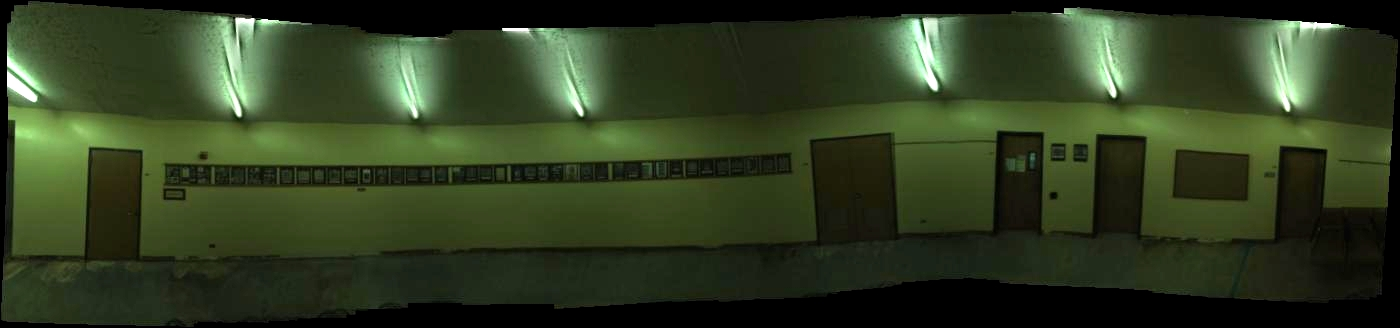
\includegraphics[width=3in]{panoMy.jpg}
  \caption{Image mosaicing. }
  \label{fig:mosaic}
\end{figure}


When images are taken of a plane from arbitrary overlapping positions,
they are related by homography \cite{hz}. Thus, existing
homography-based image mosaicing algorithms are applicable
\cite{brown2007automatic}. However, errors can compound when long
chains of images are mosaiced together using these approaches. For
example, a pixel in the $n$th image in the chain must be translated
into the first image's coordinates by multiplying by the $3\times3$
matrix $H_1 H_2 H_3 ... H_n$. Any error in one of these homography
matrices is propagated to all further images until the chain is
broken. For some chains of images this can happen almost immediately
due to erroneous correspondence matches and the resulting image mosaic
is grossly misshapen.

Figure \ref{fig:mosaic} shows the output of the AutoStitch software
package which does homography-based image mosaicing. This plane is
nearly a best-case scenerio with many features spread uniformly across
it. Even so, the mosaicing produces errors that causes straight lines
to appear as waves on the plane. This image was generated after
careful hand tuning. Many planes that had fewer features simply
failed. This led to the conclusion that image mosaicing is not a
robust enough solution for reliably texture mapping our dataset.

\subsection{Image-Based 3D Localization Refinement}

\begin{figure}
  \centering
  
\includegraphics[width=3in]{Graph_crop.pdf}
  \caption{Using the graph-based localization refinement algorithm
    from [11] suffers from the problem of compounding errors. }
  \label{fig:graph}
\end{figure}

Another approach is to refine the camera matrices using image
correspondences to guide the process. Each image's camera matrix has 6
degrees of freedom. Previous work has attempted to refine camera
matrices by solving a non-linear optimization problem
\cite{liu2010indoor}. This process is specific to the backpack system
which generated our dataset, as it must be run during backpack
localization\cite{liu2010indoor,chen2010indoor}. Unfortunately, this
approach suffers from a similar error propagation problem shown in
Figure \ref{fig:graph}. In our new approach, we also refine the
placement of images using image correspondences. However, we do so in
two dimensions on the plane whereas this previous work did so over all
6 degrees of freedom. Refining in two dimensions on the plane is less
flexible in that it does not address projection errors, however, it
provides noticeable benefits while avoiding the error propagation
problem.


\section{Our Approach Overview}
Our approach begins 
with the projection of all our images onto
separate copies of our plane, such that no projected data is covered
and lost. Tis is done by discretizing the plane into an arbitrary density of points, and projecting each point into the image plane using the camera matrix $P_i$. We then perform a series of preprocessing steps to rotate
and shift each image's projection such that its overlapping regions
with other projections are as seamless as possible. From here, we assign textures to our planes
using one of two methods, dependent on whether they are wall planes or
ceiling/floor planes. The reasoning for this is explained in section
\ref{sec:whydifferent}. Lastly, we apply two post-processing steps to smooth out
any remaining seams.

\subsection{Hough Transforms}
Our first step is to use Hough transforms to rotate
the projected images such that any strong near-vertical features are made completely vertical. This is effective for indoor modeling, since many indoor
scenes contain strong vertical lines from features such as doors, wall
panels, or rectangular frames.


\subsection{Localization Refinement}
Our next step is to try and fix misalignment between overlapping images.
We do this by fixing
the locations in 2D. First we find corresponding points between all
pairs of overlapping images using SIFT matches
\cite{lowe1999object}. An illustration of this is given in Figure
\ref{fig:matches}. The SIFT matches allow us to determine feature-based $x$ and $y$ distances between two images on the plane, which we can compare against the $x$ and $y$ distances provided by the camera matrices. With these data points, we can reevaluate where each image should be projected.

\subsubsection{Robust SIFT Distances using RANSAC}

First we need to ensure that the SIFT-based distances are
reliable. Since SIFT matches frequently include outliers, the RANSAC
framework \cite{fischler1981random} is used for a robust estimate of
the $x$ and $y$ distances between the two images. The RANSAC framework
will attempt to build a consensus among the SIFT matches about what
the true $x$ and $y$ distance is between the two images while ignoring
the influence of outliers that may skew the results. The framework
handles the consensus-building machinery, and only requires that two
functions be specified: the fitting function and the distance
function. These functions are called for random subsets of the SIFT
matches until the best set of inliers is found. For this application,
the fitting function simply finds the average distance between
matches. If the matches are exactly correct and the image is frontal
and planar then the distances for various SIFT feature matches should
be the same. Our distance function for a pair of points is the
difference between those points' SIFT match distance and the average
distance computed by the fitting function. We specified a 10 pixel
outlier threshold to the framework. This means that a SIFT match is
labeled as an outlier if its $x$ and $y$ distance is not within 10
pixels of the average distance computed by the fitting function.

\subsubsection{Refining Image Positions using Least Squares}

There are a total of $M^{2}$ possible pairs of images, however we can
only measure distances between images that overlap at SIFT feature
points. Given these distances and the original image location
estimates, we solve a least squares problem ($\textrm{min}_{\beta}
||\beta X - y||_2^2 $) to estimate the correct location of the images
on the plane. The vector $\beta$ of unknowns are the correct $x$ and
$y$ locations of each image on the plane from $1 \dots M$. Finding the
correct $x$ and $y$ locations are independent from one another so we
will only consider the $x$ locations:

% Draw least squares problem here.

\[\beta =
\begin{pmatrix}
  x_1, & x_2, & x_3, & \cdots & x_{M-1}, & x_M
\end{pmatrix}
\]

The matrix $X$ is constructed with one row for each pair of images
with measured distances produced by the SIFT matching stage. A row in
the matrix has a $-1$ and $1$ in the columns corresponding to the two
images in the pair. For example, the matrix below indicates that we
generated a SIFT-based distance between images 1 and 2, images 1 and
3, images 2 and 3, etc.

\[
X =
\begin{pmatrix}
  -1 & 1 & 0 & \cdots & 0 & 0\\
  -1 & 0 & 1 & \cdots & 0 & 0\\
  0 & -1 & 1 & \cdots & 0 & 0\\
  \vdots  & \vdots & \vdots & \ddots & \vdots  & \vdots\\
  0 & 0 & 0 & \cdots & 1 & 0 \\
  0 & 0 & 0 & \cdots & -1 & 1 \\
  1 & 0 & 0 & \cdots & 0 & 0 \\
\end{pmatrix}
\]

If only relative distances between images are included then there is
no way to determine the absolute location of any of the images and the
matrix becomes rank deficient. To fix this we choose the first image
to serve as the anchor for the rest, meaning all the absolute
distances are based on its original location. This is done by adding a
row with a $1$ in the first column and the rest zeros.

Finally, the observation vector $y$ is constructed using the
SIFT-based distances generated earlier in the matching stage. The
distances are denoted as $d_1 \dots d_N$ for $N$ SIFT-based
distances. The last element in the observation vector is the original
location of the first image determined by the localization algorithm.

\[
y^T =
\begin{pmatrix}
  d_{1,2}, &d_{1,3}, &d_{2,3}, &\hdots &d_{N-2,N-1}, &d_{N-1,N}, &x_1
\end{pmatrix}
\]

The $\beta$ that minimizes $||\beta X - y||_2^2$ tells us a set of
image locations on the plane that best honors all the SIFT-based
distance measurements between images. A similar problem is solved for
the $y$ dimension. In practice there are often cases where there is a
break in the chain of images, meaning that no SIFT matches were found
between one segment of the plane and another. In this case we add rows
to the $X$ matrix and observations to the $y$ vector that contain the
original $x$ and $y$ distance estimates generated by the localization
algorithm. Another way to do this is to add rows for all neighboring
pairs of images and solve a weighted least squares problem where the
SIFT distances are given a higher weight i.e. 1, and the distances
generated by the localization algorithm are given a smaller weight
i.e. 0.01.

At this point we now have our target plane associated with a list of
images as well as their rotated and shifted projections upon the
plane. We are ready to begin assigning these projections to areas of
our plane for texturing.



\subsection{Ceiling/Floor Texturing vs. Wall Texturing}
\label{sec:whydifferent}
The backpack modeling system, as described in Section
\ref{sec:backpackHardware}, was designed to prioritize for texturing
walls. As mentioned previously, the backpack contains two fisheye
cameras, one aimed directly to the left of the backpack operator, and
one aimed directly to the right. Thus, in order to texture the ceiling
above where the operator walked, images from both cameras must be
combined, with their boundaries meeting overhead. Unlike walls, where
one image generally spans the entire height of a wall, two images are
required to span the width of a ceiling. Even more problematic, the
floor beneath the backpack is physically obscured by the operator's
body, and thus must be textured by images taken from behind the
operator or from the side. This problem of distant cameras at poor
angles is compounded by the fact that the operator's data acquisition
path attempts to fully scan each wall, but not necessarily the
entirety of a floor or ceiling. This means that large swaths of floors
and ceilings are never walked directly over or under, and thus must be
textured by sidelong images taken from further distances and at
oblique angles. These effects are shown in the following figure.

In short, these factors mean that wall planes are generally associated
with a multitude of upright, uniform images, from a relatively close
distance and taken head-on at regular intervals, while floors and
ceilings are associated with images taken from all manner of
orientations and distances. This major difference suggests we employ
two strategies, one tailored for each scenario.


\subsection{Texturing Walls}
Because wall images tend to all be fairly good candidates for
texturing due to their orientation and location, our goal is less
about determining the best images, and more about selecting a set of
images that together form the most seamless texture.

\subsubsection{Cost Functions}

In order to objectively decide which set of images accomplishes this,
we need to decide on an overall cost function. As our goal is to reduce
the seams that occur where two images meet, a simple cost function is
the sum of squared pixel differences in overlapping regions between
every pair of images. This encourages image boundaries to occur in
featureless areas, such as bare walls, on in areas where images are
very well aligned.

Another possible cost function is edge energy, i.e. the sum of the
smoothed gradient of the blended seam regions. Minimizing this
encourages image boundaries to be placed in featureless areas even
more than the first cost function. For the results shown throughout
this paper, the first cost function was used, as the regular
occurrence of featureless areas was not guaranteed in our datasets.

\subsubsection{Image Selection}

Now that we have a cost function defined, we need to mechanically
select the set of images for which the overall cost function is
minimized. Since we aim to cover the entirety of our plane, our
problem is to minimally cover a polygon(our plane) using other
polygons of arbitrary geometry (our image projections), with the added
constraint of minimizing our cost function. This is a complex problem,
though it can be generalized to a number of graph coverage problems,
as depicted in figure X. Returning again to the optimality of our
situation when texturing walls however, we can make a quick
simplification for the sake of efficiency. Given that our wall-texture
candidate images were all taken from a head-on angle, and assuming only minor rotations were made earlier, we can reason
that their projections onto the plane are approximately
rectangular. By discarding any excess texture and cropping them
all to be rectangular, our problem becomes the conceptually simpler
problem of filling a polygon with rectangles, such that the sum of all
edge costs between each pair of rectangles is minimal. An additional
benefit of working with rectangular units is that borders between any
two distinct images in our final texture will be either horizontal or
vertical. Since most environmental features inside buildings are horizontal
or vertical, any seams in our texture will intersect them miniimally
and be less noticeable.

By taking one more shortcut we can simplify our problem down even
further. Since care is taken such that our wall images contain the
floor-to-ceiling range of walls, we generally do not have any wall
images such that one should be projected vertically above the
other. In essence, we need only to ensure horizontal coverage of our
planes, as our images provide full vertical coverage. We can thus
construct a Directed Acyclic Graph (DAG) from the images, again with
edge costs defined by our cost function above, and solve a simple
shortest path problem to find an optimal subset of images with regard
to the cost functions.

\begin{figure}
  \centering
  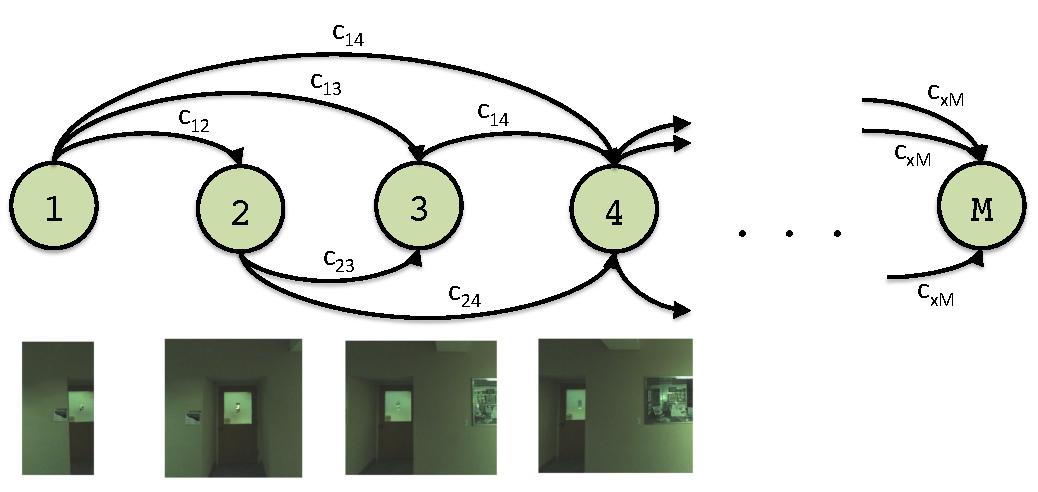
\includegraphics[width=3in]{DynProg.pdf}
  \caption{Image Selection is done by constructing a graph of sorted
    images. Then we solve a shortest path problem where the edge
    weights represent the cost of a seam between two overlapping
    images.}
  \label{fig:DynProg}
\end{figure}

Figure \ref{fig:DynProg} demonstrates the construction of a DAG from
overlapping images of a long hallway. Images are sorted by horizontal
location left to right, and become nodes in a graph. Directed edges
are placed in the graph from left to right between images that
overlap. The weights of these edges are determined by the cost
functions discussed previously. Next, we add two artificial nodes, one
start node representing the left border of the plane, and one end node
representing the right border of the plane. The left artificial node
has directed edges with equal cost to all images that meet the left
border of the plane, and the right artificial node has directed edges
from all images that meet the right border of the plane.

We now solve the standard shortest path problem from the start node to
the end node. This provides a set of images that completely covers the
plane horizontally, while minimizing the cost of the seams between
images.

In rare cases where the vertical dimension of the plane is not entirely
covered by a chosen image, we are left with a hole where no image was
chosen to texture. Rather than reverting to a 2D-coverage problem, we
can elect to simply fill the hole by selecting images in a
greedy fashion, with respect to the same cost function.

At this point, we have mapped every location on our plane to an image
or images that were selected. Before applying these textures, we will
examine how to accomplish the same mapping for ceilings and floors.

\subsection{Texturing Ceilings and Floors}

Because the images associated with ceilings and floors are often
captured by cameras at sidelong angles, we must be conservative when
we texture map them. Since localization errors compound over distance,
we often have candidate images that project well on areas near the
camera itself, but much more poorly at the greater distances caused by
higher angles. Using entire images to minimize seams is beneficial for
wall texturing, but it becomes detrimental on ceilings and floors,
since the quality of usable texture varies greatly across any one
image. As evident in the following comparison, ceiling and floor
images often have a very low amount of optimal texture relative to the
projection size. This factor suggests that we should segment our images in some way, as many of our images contain both desired as well as undesired portions.

Such segmentation
implies smaller units of texture, which often leads to more images being
chosen and unfortunately, more boundaries between different images as
a result. This goes strongly against our approach for texturing walls,
in which we attempted to minimize the number of images chosen. Nevertheless, boundaries on
floors and ceilings are less problematic, since floors and ceilings
tend to have fewer noticeable features.

As shown in the above figure, we define
a tile length $l1$ as well as an overlap length $l2$, usually about 5
pixels for each. We then discretize our plane into rectangular tiles
$l1$x$l1$ in size. Each tile is then associated with a square
texture of size $(l1+2l2)$x$(l1+2l2)$, such that it shares a large
overlapping region with its neighboring tiles, allowing for blending afterwards. As in wall texturing, rectangles, rather than triangles, are preferred for the high prevalence of horizontal and vertical features, generally light fixtures and floor and ceiling tiles.

For the actual process of image association, we can reuse the caching method shown earlier. This method will balance selection of the best texture for each tile with some amount of image reuse. Coupled with image rotation and shifting, as well as the usage of rectangles instead of triangles, we end with a much more seamless texture, even without any blending applied yet, as seen below.

\subsection{Blending}
Though our preprocessing steps and image selection attempts above
attempted to minimize all mismatches between images, there are often
cases, where due to geometry or projection inaccuracies, we simply
have unavoidable discontinuities. These can however be partially
treated by applying alpha blending over our seams.  Whether the units
we are blending are rectangularly-cropped images for walls, or
rectangular units for ceilings/floors, we can apply the same blending
procedure.

Our alpha blending technique is widely used, and blends pixels
linearly across overlapping regions. For each pixel within an
overlapping region, we simply multiply its intensity (by a factor from 0 to
1), based on its distance from the image's border, with a cap set at some maximum blending distance. In this way, we
interpolate between two overlapping images, providing a gradual
transition between them. Increasing the overlapping and blending distance
results in a smoother transition, but can also result in more
blurriness. The final output is shown in Figure X.


{\small \bibliographystyle{ieee} \bibliography{egbib} }


\end{document}
